\documentclass{article}
\usepackage[utf8]{inputenc}
\usepackage{tasks}
\usepackage{kotex}
\usepackage{amsthm}
\usepackage{amssymb}
\usepackage{hyperref}
\usepackage{mathtools}
\usepackage{cleveref}
\usepackage{lipsum}
\usepackage{polynom}
\usepackage{array}
\usepackage{enumitem}
\usepackage{authblk}
\usepackage{listings}
\usepackage{caption}
\usepackage{setspace}
\usepackage{pgfplots}
\usepackage{graphicx}

\newtheorem{definition}{Definition}

\lstset{
    frame=single,
    language=C++,
    numbers=left,
}

\graphicspath{ {./} }

\begin{document}
    \title{%
        POINTER 알고리즘 세미나 \\
        \large 제 2강 - 자료 구조 (Data structure)}
    \author{Kim Jun Hyeok}
    \affil{Kangwon Science Highschool}
    \maketitle
    \linespread{1.25}
    \section{개요}
        \subsection{자료 구조의 필요성}
        다음과 같은 3가지의 연산을 빠르게 하기 위해서 등장함.
        \begin{itemize}
            \item 삽입 (Insertion)
            \item 삭제 (Deletion)
            \item 탐색 (Search)
        \end{itemize}
        \subsection{자료 구조의 분류}
        \paragraph{선형 자료구조} 데이터가 순차적으로 연결되어있는 방법으로 표현된 자료구조.
        ex) 배열, 연결 리스트, 스택, 큐등
        \begin{figure}[h]
            \centering
            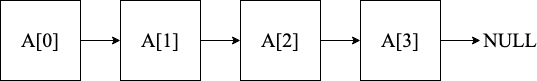
\includegraphics[width=\textwidth]{Linear_Structure.png}
            \caption{선형 자료구조의 예시: 연결 리스트(Linked list)}
            \label{}
        \end{figure}
        \newpage
        \paragraph{비선형 자료구조} 데이터가 순차적으로 연결되어있지 않은 방법으로 표현된 자료구조.
        ex) 그래프, 트리등
        \begin{figure}[h]
            \centering
            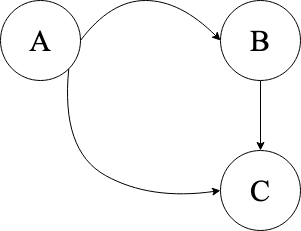
\includegraphics[scale=0.5]{Non_Linear_Structure.png}
            \caption{비선형 자료구조의 예시: 그래프(Graph)}
            \label{}
        \end{figure}
    \section{선형 자료 구조}
    \subsection{스택(Stack)}
    \paragraph{개요}
    스택(Stack) 자료 구조는 먼저 집어넣은 원소가 가장 먼저 나오게 하는 LIFO(Last-In, First-Out)형식을 따르는 자료 구조이다. \cite{cormen_2009}
    이러한 스택(Stack) 자료 구조는 동적 할당 배열(Dynamic array)로 구현할 수 있다.
    \begin{figure}[h]
        \centering
        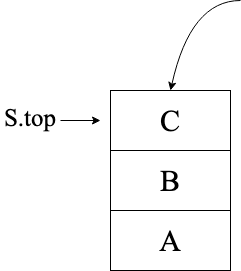
\includegraphics[scale=0.5]{Stack.png}
        \caption{스택(Stack) 자료 구조를 표현한 그림}
        \label{}
    \end{figure}
    \newpage
    \paragraph{속성}
    \begin{itemize}
        \item $top$ - 가장 최상위의 원소를 반환함.
    \end{itemize}
    \paragraph{기본 연산} 스택(Stack) 자료 구조에서 기본 연산은 다음과 같다.
    \begin{itemize}
        \item $PUSH(s)$ - $top$에 원소를 삽입함.
        \item $POP()$ - $top$에 있는 원소를 제거함.
        \item $STACK-EMPTY()$ - 스택이 비었는지 확인함.
    \end{itemize}
    \paragraph{구현} C++ 11 표준안을 기준으로 \texttt{std::stack}을 통해서 사용할 수 있음.
    \subsection{큐(Queue)}
    \paragraph{개요}
    큐(Queue) 자료 구조는 먼저 집어넣은 원소가 나중에 나오게 하는 FIFO(First-In, First-Out)형식을 따르는 자료 구조이다. \cite{cormen_2009}
    \begin{figure}[h]
        \centering
        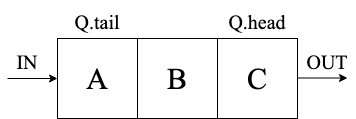
\includegraphics[scale=0.5]{Queue.png}
        \caption{큐(Queue) 자료 구조를 표현한 그림}
        \label{}
    \end{figure}
    \paragraph{속성}
    \begin{itemize}
        \item $tail$ - 가장 처음에 삽입된 원소를 반환함.
        \item $head$ - 가장 나중에 삽입된 원소를 반환함.
    \end{itemize}
    \paragraph{기본 연산} 큐(Queue) 자료 구조에서 기본 연산은 다음과 같다.
    \begin{itemize}
        \item $ENQUEUE(s)$ - $tail$에 원소를 삽입함.
        \item $DEQUEUE()$ - $head$에 있는 원소를 제거함.
    \end{itemize}
    \bibliographystyle{IEEEtranS}
    \bibliography{2_Data_structure}
\end{document}